\textbf{Diseño del Eje de Aireación}

Para conocer las dimensiones reales del eje que se ve a utilizar el sistema de aireación, se usará la siguiente fórmula:

\begin{center}
    $D=\sqrt[3]{\frac{32*N}{\pi}*\sqrt{(K_t*\frac{M}{s'n})^2+ \frac{3}{4}*(\frac{T}{S_y})^2}}$
\end{center}

Se propone utilizar el acero ANSI 1045, porque es un acero de fácil adquisición, además de ser fácilmente maquinable,  tiene las siguientes características:

\begin{table}[h]
\begin{center}
\caption{Propiedades Acero ANSI 1045}
\begin{tabular}{| c | c | }
 \\ 
Característica & Magnitud \\ \hline
Dureza & $HB=179$  \\
Esfuerzo Máximo & $\sigma_r = 91.4 ksi$ \\
Esfuerzo de Fluencia & $S_y = 76.9 ksi$ \\
Elongación & $e=12\%$ \\ 
Reducción de área & $R_a=35\%$ \\ 
Maquinabilidad & $EF =55\%$ \\ 
    \end{tabular}
        \label{tab:A1045}
        \end{center}
\end{table}

El valor de la resistencia a la fatiga será vital a la hora de calcular el diámetro real de los ejes de transmisión, el cual se calcula:

\begin{center}
    $s'n =  sn*C_m*C_{st}*C_r*C_s$
\end{center}

El valor de sn se determina en función de la tabla siguiente (Figura \ref{fg:Res_fat}). 

De la gráfica se puede determinar que el valor a la fatiga teórico es de:

\begin{center}
    $sn=25 ksi$
\end{center}

Se sugiere un factor de material \cite{Mott}:
$C_m= 1$

Y un factor de esfuerzos:
$C_{st}=1$

Para determinar el Factor de confiabilidad se utiliza la siguiente tabla (Figura \ref{fg:Fac}). 

\begin{figure}[h]
    \centering
        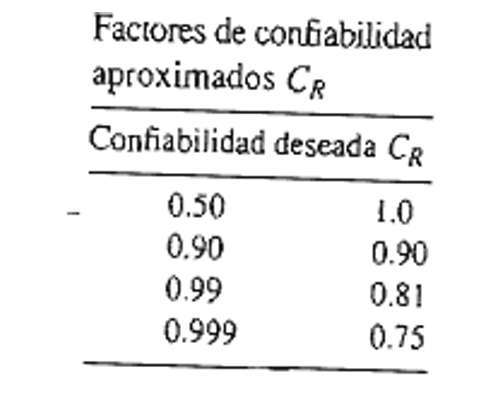
\includegraphics[scale=0.6]{images/Capitulo 4/s5/Factores de confiabilidad.png}
        \caption{Factores de confiabilidad}\cite{Mott}
    \label{fg:Fac}
\end{figure}

Se selecciona un grado de fiabilidad de 0.99, por lo que:

$C_r := 0.81$

Finalmente, para determinar el factor de tamaño se debe estimar el tamaño del eje, en función de la siguiente tabla (Figura \ref{fg:diseño}). 

\begin{figure}[h]
    \centering
        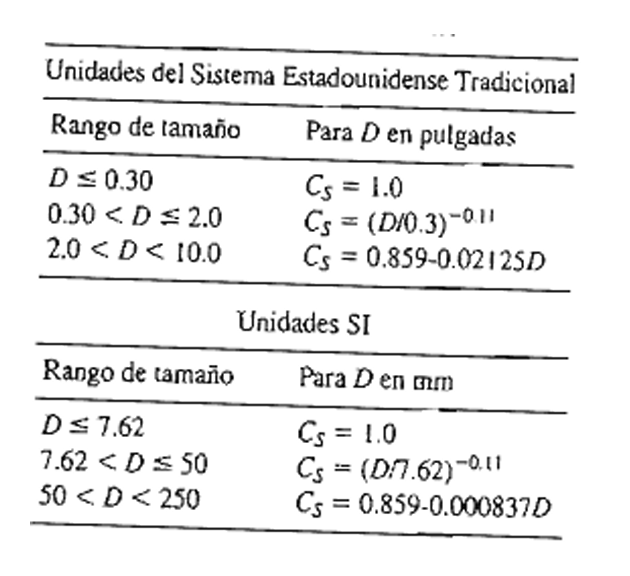
\includegraphics[scale=0.6]{images/Capitulo 4/s5/Factores de diseno aproximado.png}
        \caption{Factores de dise\~{n}o aproximado}\cite{Mott}
    \label{fg:diseño}
\end{figure}

Se estima que el eje tendrá un diámetro entre $0.3 in < D < 2.0 in $, se propone un valor máximo de 2 in. 

\begin{center}
    $D_{max}= 2 in$
\end{center}

Por lo que el factor de tamaño $C_s$ es:

\begin{center}
    $C_s = (\frac{D_{max}}{0.3})^{-0.11} = 0.812 $
\end{center}

Teniendo en cuenta todos estos factores, se procede a a reemplazar los en la fórmula de la resistencia de la fatiga real:

\begin{center}
    $s'n =  25 ksi*(1)*(1)*(0.81)*(0.812) = 16.44 ksi $
\end{center}

Ya determinado el factor de fatiga real, se procede a determinar las fuerzas que actúan sobre el eje, sabiendo que tendrá 3 palas y estarán 2 de un lado y una del otro, se tiene:

1 Pala(Figura \ref{fg:1pala}). 

\begin{figure}[h]
    \centering
        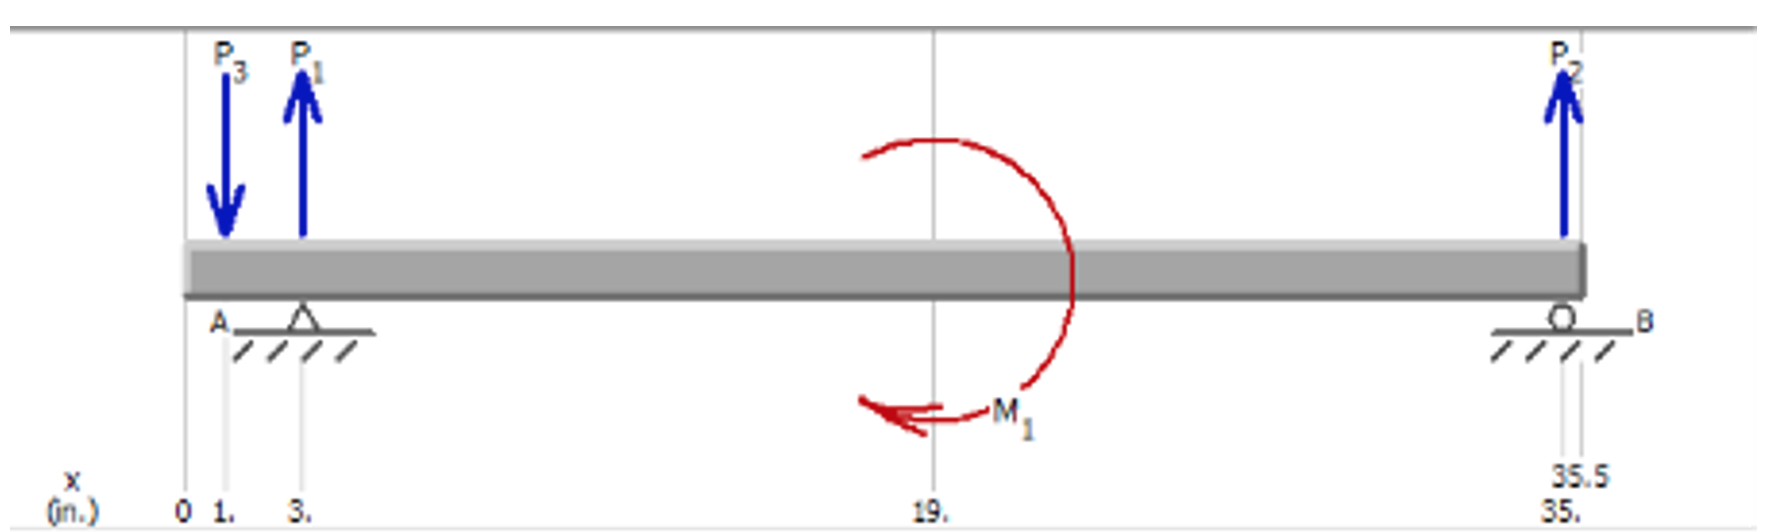
\includegraphics[scale=0.4]{images/Capitulo 4/s5/1 pala.png}
        \caption{Fuerzas del lado del eje con 1 pala}
    \label{fg:1pala}
\end{figure}

2 Palas(Figura \ref{fg:2palas}). 

\begin{figure}[h]
    \centering
        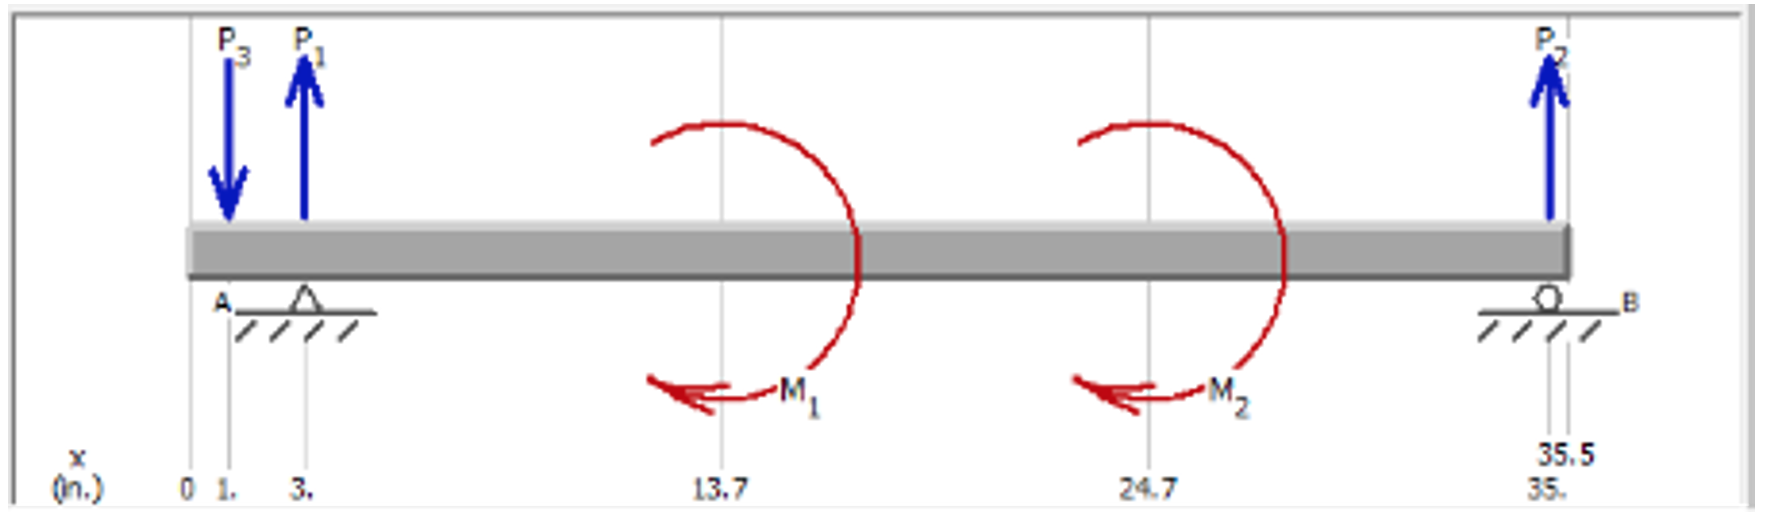
\includegraphics[scale=0.4]{images/Capitulo 4/s5/2 palas.png}
        \caption{Fuerzas del lado del eje con 2 palas}
    \label{fg:2palas}
\end{figure}

Donde: \\
P1 y P2 son las reacciones de la barra a su soportes. \\
P3 es la fuerza generada por la tensión de la banda 3V. \\
M1 con una pala y M1 y M2 representan el momento de torsión generado por las palas al instante de hacer girar la materia orgánica. \\ 

Para determinar  la fuerza generada por la tensión de la banda P3, se tiene:
\begin{center}
    $F_c = \frac{2T}{D}$
\end{center}

Donde: \\
T: es el torque al que se somete la polea \\
D: es e diámetro máximo de la polea \\

Si se tiene que:

\begin{center}
    $ T = 40 Nm$ \\
    $D_{polea}=2.5 in = 0.0635 m$
\end{center}

Entonces se tiene que la fuerza $F_c$ es:

\begin{center}
    $F_c = \frac{2*40 Nm}{0.0635m} = 1259.84 N $
\end{center}

Por lo que los diagramas de fuerzas quedan de la siguiente manera:

%\newpage
1 Pala(Figura \ref{fg:1palaF}). 

%\newpage 
2 Palas(Figura \ref{fg:2palasF}). 

Como se busca tener un eje de diámetro constante se toma el momento flexionante más grande de las gráficas, por lo que:

\begin{center}
    $M= 47.76 Nm$
\end{center}

Se define $K_t = 2.5$ de acuerdo a los valores propuestos para perfiles redondeados \cite{Mott}.

Y se selecciona un factor de seguridad $N=3$.

Con los datos obtenidos se procede a calcular el diámetro mínimo para el eje de transmisión,  sustituyendo todos los valores anteriores se tiene que:

\begin{center}
    $D=\sqrt[3]{\frac{32*3}{\pi}*\sqrt{(2.5*\frac{47.76 Nm}{16.64 ksi})^2+ \frac{3}{4}*(\frac{40 Nm}{76.9ksi})^2}} = 1.25 in$
\end{center}

Se puede ver que el diámetro mínimo de diseño es de $D=1.25 in$, sin embargo al ser el mínimo teórico calculado y no tomar en cuenta el posicionamiento del los rodamientos y las perforaciones que se le harán para poder sujetar las palas de agitación, se decidió seleccionar un diámetro $D=1.5 in$.

Esta medida permite mantener un diámetro efectivo de 1.25 pulgadas, a su vez colocar los rodamientos en su posición fácilmente.

Con estos datos calculados, se procedió a diseñar el siguiente eje de transmisión (Figura \ref{fg:eje}). 

\begin{figure}[h]
    \centering
        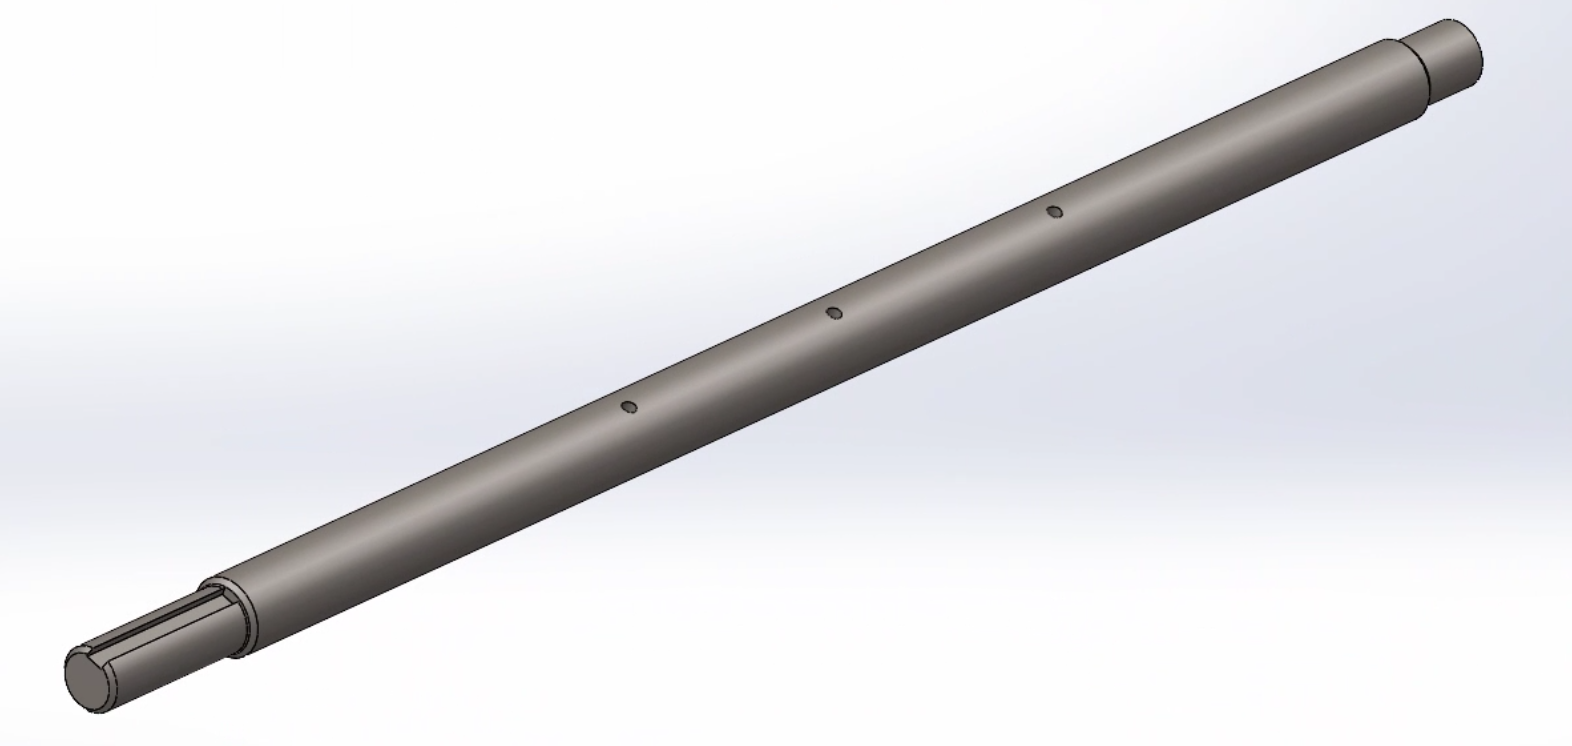
\includegraphics[scale=0.45]{images/Capitulo 4/s5/Eje Trituracion.png}
        \caption{Diseño de eje}
    \label{fg:eje}
\end{figure}
